\documentclass{article}
\usepackage[UTF8]{ctex}
\usepackage[left=2cm,right=2cm,top=1.5cm,bottom=1.5cm]{geometry}
\usepackage{listings}
\usepackage{xcolor}
\usepackage{fontspec}
\usepackage{amsmath}
\usepackage{tikz}
\usetikzlibrary{calc}
\usepackage[thmmarks,amsmath]{ntheorem}
\setmonofont{Consolas}

\begin{document}
	\title{HW 4}
	\author{肖桐 PB18000037}
	\date{2020 年 11 月 4 日}
	\maketitle

	\newtheorem*{solution}{解}

	\begin{solution}\textnormal{\textbf{1.}}
		(a). \newline
		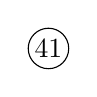
\begin{tikzpicture}[level distance=15mm,
							every node/.style={circle,draw,inner sep=1pt},
							level 1/.style={sibling distance=20mm},
							level 2/.style={sibling distance=10mm}]
			\node[circle, draw]{$41$};
		\end{tikzpicture}
		\newline
		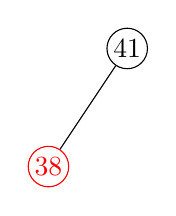
\begin{tikzpicture}[level distance=15mm,
							every node/.style={circle,draw,inner sep=1pt},
							level 1/.style={sibling distance=20mm},
							level 2/.style={sibling distance=10mm}]
			\node[circle, draw]{$41$}
				child{node[color=red!]{$38$}}
				child[missing];
		\end{tikzpicture}
		\newline
		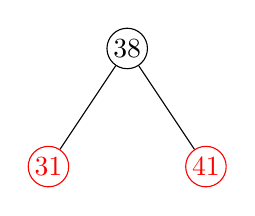
\begin{tikzpicture}[level distance=15mm,
							every node/.style={circle,draw,inner sep=1pt},
							level 1/.style={sibling distance=20mm},
							level 2/.style={sibling distance=10mm}]
			\node[circle, draw]{$38$}
				child{node[color=red!]{$31$}}
				child{node[color=red!]{$41$}};
		\end{tikzpicture}
		\newline
		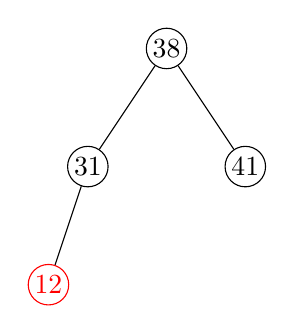
\begin{tikzpicture}[level distance=15mm,
							every node/.style={circle,draw,inner sep=1pt},
							level 1/.style={sibling distance=20mm},
							level 2/.style={sibling distance=10mm}]
			\node[circle, draw]{$38$}
				child
				{	
					node{$31$}
						child
						{
							node[color=red!]{$12$}
						}
						child[missing]
				}
				child{node{$41$}};
		\end{tikzpicture}
		\newline
		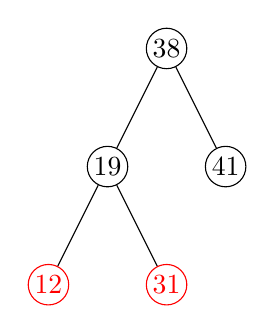
\begin{tikzpicture}[level distance=15mm,
							every node/.style={circle,draw,inner sep=1pt},
							%level 1/.style={sibling distance=20mm},
							sibling distance=15mm]
			\node[circle, draw]{$38$}
				child
				{	
					node{$19$}
						child
						{
							node[color=red!]{$12$}
						}
						child
						{
							node[color=red!]{$31$}
						}
				}
				child{node{$41$}};
		\end{tikzpicture}
		\newline
		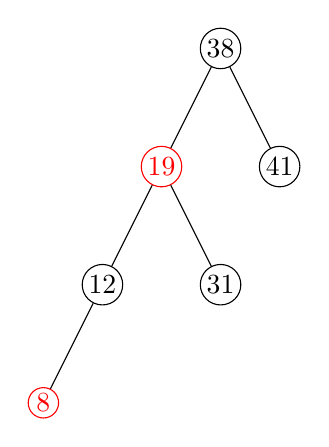
\begin{tikzpicture}[level distance=15mm,
							every node/.style={circle,draw,inner sep=1pt},
							%level 1/.style={sibling distance=20mm},
							sibling distance=15mm]
			\node[circle, draw]{$38$}
				child
				{	
					node[color=red!]{$19$}
						child
						{
							node{$12$}
								child
								{
									node[color=red!]{$8$}
								}
								child[missing]
						}
						child
						{
							node{$31$}
						}
				}
				child{node{$41$}};
		\end{tikzpicture}
		\newline
		(b). 删除$8$:
		\newline
		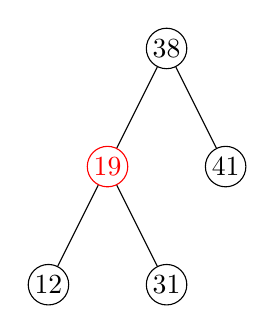
\begin{tikzpicture}[level distance=15mm,
							every node/.style={circle,draw,inner sep=1pt},
							%level 1/.style={sibling distance=20mm},
							sibling distance=15mm]
			\node[circle, draw]{$38$}
				child
				{	
					node[color=red!]{$19$}
						child
						{
							node{$12$}
						}
						child
						{
							node{$31$}
						}
				}
				child{node{$41$}};
		\end{tikzpicture}
		\newline
		删除$12$:
		\newline
		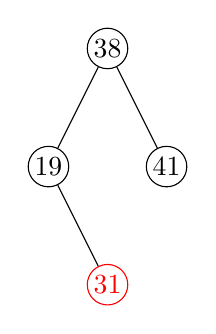
\begin{tikzpicture}[level distance=15mm,
							every node/.style={circle,draw,inner sep=1pt},
							%level 1/.style={sibling distance=20mm},
							sibling distance=15mm]
			\node[circle, draw]{$38$}
				child
				{	
					node{$19$}
						child[missing]
						child
						{
							node[color=red!]{$31$}
						}
				}
				child{node{$41$}};
		\end{tikzpicture}
		\newline
		删除$19$:
		\newline
		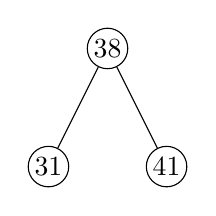
\begin{tikzpicture}[level distance=15mm,
							every node/.style={circle,draw,inner sep=1pt},
							%level 1/.style={sibling distance=20mm},
							sibling distance=15mm]
			\node[circle, draw]{$38$}
				child
				{	
					node{$31$}
				}
				child
				{
					node{$41$}
				};
		\end{tikzpicture}
	\end{solution}
	\begin{solution}\textnormal{\textbf{2.}}
		(a). 可以将区间树的所有区间合并到一个数轴上, 每个区间的每个端点都在数轴上取相应的端点.
		(如区间$[0, 3]$, 则在数轴上取端点$0, 3$).\newline
		假设最大重叠点所在区间为$[\alpha, \beta]$, 则显然区间$[\alpha, \beta]$内所有点都是最大重叠点, 端点$\alpha$和$\beta$也是最大重叠点.\newline
		(b). 可以采用$(a)$中的思路, 将所有区间合并到一个数轴上. 具体方法为将原红黑树中所有区间节点复制下来, 将所有区间的端点分别打包为一个结构体.
		使用一个$int$值标识端点数值大小, 再使用一个$int$标识是左端点还是右端点. 然后对该结构体数组进行排序.\newline
		最后只需要对排好序的数组扫描一遍, 每遇到左端点$depth + 1$, 遇到右端点$depth - 1$. 最后取最大的$depth$对应的端点值即可.
	\end{solution}
	\begin{solution}\textnormal{\textbf{3.}}
		(a). 问题在于将$x$的所有直接子节点插入根节点过程中, 要将$x$的所有直接子节点的$p$指针置为$NIL$,
		这显然会与$x$的度数有关, 不能在$O(1)$的时间内完成.\newline
		(b). 第$5-7$行复杂度为$O(c)$, 第$8$行复杂度为$O(x.degree)$, 因此总的复杂度为$O(c + x.degree)$.
	\end{solution}
\end{document}